%%%%%%%%%%%%%%%%%%%%%%%%%%%%%%%%%%%%%%%%%%%%%%%%%%%%%%%
%% Engineer & Master Thesis, LaTeX Template          %%
%% Copyleft by Piotr Woźniak & Artur M. Brodzki      %%
%% Faculty of Electronics and Information Technology %%
%% Warsaw University of Technology, Warsaw, 2019     %%
%%%%%%%%%%%%%%%%%%%%%%%%%%%%%%%%%%%%%%%%%%%%%%%%%%%%%%%

\documentclass[
    left=2.5cm,         % Sadly, generic margin parameter
    right=2.5cm,        % doesnt't work, as it is
    top=2.5cm,          % superseded by more specific
    bottom=3cm,         % left...bottom parameters.
    bindingoffset=6mm,  % Optional binding offset.
    nohyphenation=false % You may turn off hyphenation, if don't like. 
]{eiti/eiti-thesis}

\usepackage[polish]{babel}
\usepackage[
    backend=bibtex,
    style=ieee
]{biblatex}
\usepackage{csquotes}
\usepackage{textgreek}

\graphicspath{{img/}}             % Katalog z obrazkami.
\addbibresource{bibliografia.bib} % Plik .bib z bibliografią

%----------------------------------------
% Twierdzenia i definicje;
% tutaj ew. tłumaczymy te terminy
% na inne języki
%----------------------------------------
\newtheorem{theorem}{Twierdzenie}
\newtheorem{lemma}{Lemat}
\newtheorem{corollary}{Wniosek}
\newtheorem{definition}{Definicja}
\newtheorem{axiom}{Aksjomat}
\newtheorem{assumption}{Założenie}

%----------------------------------------
% Spis rysunków, tablic i załączników;
% tutaj ew. tłumaczymy te terminy
% na inne języki
%----------------------------------------
\AtBeginDocument{
    \renewcommand{\listfigurename}{Spis rysunków}
    \renewcommand{\listtablename}{Spis tabel}
    \renewcommand{\tablename}{Tabela}
}

\begin{document}

%--------------------------------------
% Strona tytułowa
%--------------------------------------
\MasterThesis % dla pracy inżynierskiej mamy \EngineerThesis
\title{
    SmartPark
}
\engtitle{ % Tytuł po angielsku do angielskiego streszczenia
    SmartPark
}
% TODO: Dodajcie swoje indeksy plz.
\subject{Wieloagentowe Systemy Decyzyjne}
\author{Jan Dubiński | 271165}
\secondAuthor{Joanna Kaleta | 271181}
\thirdAuthor{Aleksander Ogonowski | 267381}
\fourthAuthor{Maria Oniszuczuk | 271199}
\fifthAuthor{Kornel Szymczyk | 267778}
\date{\the\year}
\maketitle

%--------------------------------------
% Spis treści
%--------------------------------------
repozytorium git: \url{https://github.com/Jot-De/WSD/}

\hfill \break

\thispagestyle{empty}
\tableofcontents

%--------------------------------------
% Rozdziały
%--------------------------------------
\newpage
\section{Opis problemu}
\newpage
\section{Słowny opis koncepcji systemu}

Proponowanym przez nas rozwiązaniem problemu omówionego w punkcie pierwszym jest SmartPark - system wieloagentowy ułatwiający znalezienie miejsca parkingowego, który pozwoli na znaczną redukcję liczby krążących w jego poszukiwaniu samochodów.

System będzie składać się z sieci parkingów oraz aplikacji mobilnej dla kierowców pojazdów. Przy wykorzystaniu aplikacji, użytkownik będzie mógł zrealizować wyszukanie oraz nawigację do jak najbliższego parkingu po wcześniejszym określeniu preferencji dotyczącej jego typu (płatny/bezpłatny).  System zapewni również równomierne rozłożenie zajętości parkingów poprzez odpowiednie propozycje. Zrównoważony powinien zostać cel kierowcy jakim jest znalezienie najbliższego parkingu i jak najbardziej równomierne zapełnianie wszystkich parkingów. Kluczowe jest tutaj unikanie sytuacji, gdy  jeden parking został zapełniony,a pozostałe będą puste.

Każde miejsce parkingowe powinno zostać wyposażone w czujniki ultradźwiękowe wykrywające zajętość miejsca oraz kamerę identyfikującą konkretny pojazd. W przypadku zwolnienia miejsca powinna podnosić się blokada uniemożliwiająca wjazd niezgłoszonemu samochodowi. Każdy parking agreguje konkretną liczbę miejsc postojowych na przykład na odcinku określonej ulicy i posiada informacje o ich zajętości. Każde miejsce parkingowe po zwolnieniu wysyła adekwatną informację do parkingu, do którego przynależy, dzięki czemu może on zgłosić chęć przyjęcia następnego kierowcy. Również gdy kierowca zgłosi chęć parkowania i kierowany jest do określonego parkingu, zwiększa się wtedy zajętość i parking oczekuje na kierowcę przez pewien ustalony czas, nie przyjmując kolejnych kierowców, jeśli brak jest wolnych miejsc lub parkingi wypełniają się nierównomiernie. Dzięki temu mamy pewność, że po dojechaniu na parking znajdziemy wolne miejsce. Gdy kierowca podjedzie do miejsca na przydzielonym parkingu i zostanie poprawnie zidentyfikowany przez kamerę poprzez numer rejestracyjny, blokada opuszcza się, kierowca parkuje na miejscu postojowym, a miejsce informuje parking o jego prawidłowym zajęciu, zwiększając zajętość jego aż do chwili opuszczenia miejsca przez pojazd. Przydzielony parkingu docelowo powinien być oznaczony np korzystając z Open Street Map jako region do którego prowadzony jest kierowca.

System zakłada współistnienie dwóch typów parkingów : płatnych  i bezpłatnych wyszukiwanych zgodnie z preferencjami kierowcy, jeśli jest to aktualnie możliwe. Można założyć że parkingi płatne powstaną w centach miast, ale przez konieczność uiszczenia opłaty ich obłożenie będzie równoważne z parkingami darmowymi, znajdującymi się w mniej dogodnych miejscach.

\noindent Podczas korzystania z aplikacji można wydzielić kilka  typowych scenariuszy:


\noindent Scenariusz 1 - główny - wyszukanie miejsca parkingowego: \\
\hspace*{1cm} 1. Użytkownik deklaruje w aplikacji chęć znalezienia miejsca parkingowego. \\
\hspace*{1cm} 2. Użytkownik wybiera typ parkingu (płatny/bezpłatny). \\
\hspace*{1cm} 3. System wyszukuje parking z przynajmniej jednym wolnym miejscem w okolicy użytkownika komunikując się z pobliskimi parkingami. \\
\hspace*{1cm} 4. System proponuje parking, które użytkownik może zaakceptować. \\
\hspace*{1cm} 5. Użytkownik wybiera w aplikacji zasugerowane przez system parking. \\
\hspace*{1cm} 6. System nawiguje kierowcę do parkingu. \\
\hspace*{1cm} 7. kierowca stawia się na dowolnym miejscu parkingowym w obrębie parkingu \\

\noindent Scenariusz 2 - alternatywny do scenariusza 1 - wybór innego typu parkingu: \\
\hspace*{1cm} 1-3. Jak w scenariuszu głównym. \\
\hspace*{1cm} 4. Aplikacja wyświetla komunikat o braku wolnych miejsc parkingowych na preferowanym typie parkingu oraz propozycję najbliższego wolnego parkingu o innym typie.  \\
\hspace*{1cm} 5. Użytkownik wybiera w aplikacji zasugerowany przez system inny parking. \\
\hspace*{1cm} 6. System nawiguje kierowcę do parkingu. \\
\hspace*{1cm} 7. Kierowca stawia się na dowolnym miejscu parkingowym w obrębie parkingu \\


\noindent Scenariusz 3 - alternatywny do scenariusza 1 - użytkownik odrzuca proponowane parking \\
\hspace*{1cm} 1-4. 	Jak w scenariuszu 2 \\
\hspace*{1cm} 5.	Użytkownik nie wybiera zasugerowanego przez system parkingu. \\
\hspace*{1cm} 6. Kierowca oddala się o pewną odległość \\
\hspace*{1cm} 7. Powrót do punktu 1  scenariusza głównego.. \\


\noindent Scenariusz 4 - brak wolnych miejsc parkingowych \\
\hspace*{1cm} 1-3. 	Jak w scenariuszu głównym \\
\hspace*{1cm} 4.	Aplikacja wyświetla komunikat o braku wolnych miejsc parkingowych na każdym typie parkingu. \\
\hspace*{1cm} 5. Kierowca oddala się o pewną odległość \\
\hspace*{1cm} 6. Powrót do punktu 1 scenariusza głównego. \\

\newpage
\section{Architektura systemu}

System opiera się na dwóch rodzajach agentów
kierowców samochodów z zainstalowaną aplikacją
parkingów agregujących miejsca parkingowe

Celem kierowców jest znalezienie parkingu jak najbliżej aktualnego miejsca, najlepiej bezpłatnego.

Celem parkingów jest natomiast niedopuszczenie do zapełnienia i odpowiednie balansowanie wypełnienia pobliskich parkingów poprzez wzajemną komunikację i uzgadnianie, który parking powinien aktualnie przyjąć pojazd.

System uzgadniania miejsc nie może dopuścić do sytuacji gdy przy jednoczesnym zgłoszeniu chęci parkowania przez dwa lub więcej samochody zostaną przydzielone dwa samochody na jedno wolne miejsce parkingowe.

Miejsca parkingowe są natomiast aktorami będącymi nieaktywnymi przez znaczną większość czasu. Ich zadanie polega jedynie na wysyłaniu komunikatów do parkingu, do którego przynależą. Jest to komunikat o zajęciu i zwolnieniu miejsca przez kierowcę. Na tej podstawie parking wie ile samochodów znajduje się na nim, a ile może przyjąć. Od liczby samochodów, które parking może przyjąć należy również samochody, które zgłosiły chęć parkowania, ale jeszcze nie dojechały. Nigdy jednak nie zostaje przyjęte więcej samochodów niż liczba wolnych miejsc.

Parkingi komunikują się z kierowcami i między sobą prowadząc do optymalnego rozłożenia samochodów.

Kierowcy komunikują się z parkingami zgłaszając chęć parkowania lub odrzucając sugerowany parking. Generalnie nie ma potrzeby, aby samochody prowadziły komunikację między sobą.

\begin{figure}[!h]
    \label{fig:architektura}
    \centering 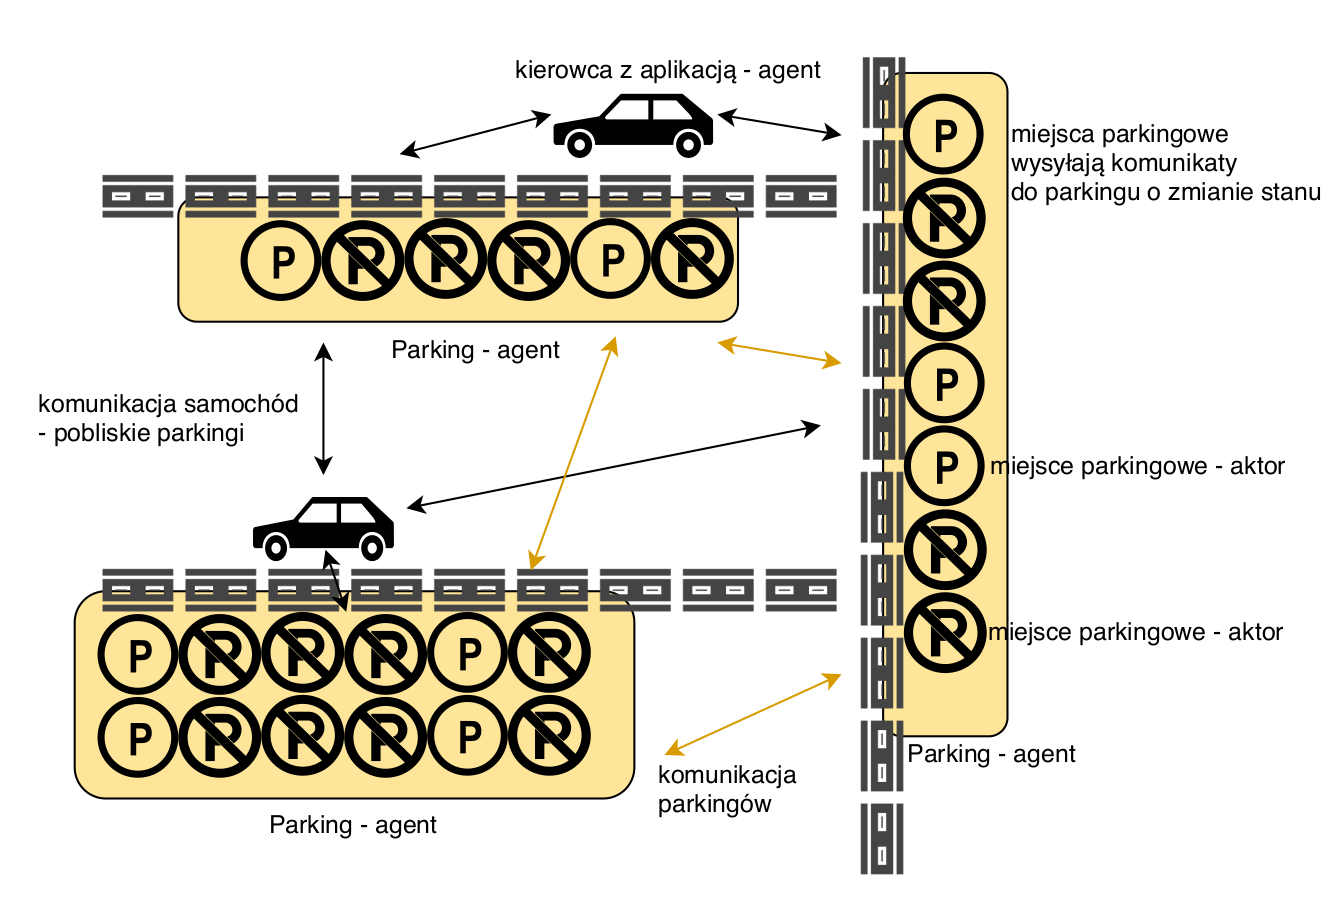
\includegraphics[width=0.8\linewidth]{archi.png}
    \caption{Architektura systemu.}
\end{figure}
\newpage
\section{Projekt systemu wieloagentowego}

\subsection{Identyfikacja ról}

\begin{enumerate}

\item Client 
\begin{itemize}
    \item zgłasza chęć zaparkowania w pobliżu udostępnionej lokalizacji
    \item akceptuje lub odrzuca propozycje wskazanego miejsca 
\end{itemize}
 
\item Parking mapper
\begin{itemize}
    \item mapuje istniejące parkingi
\end{itemize}
\item Parking Approacher
\begin{itemize}
    \item zbliża się do parkingu i wysyła komunikat z aktualną lokalizacją
\item może zrezygnować
\end{itemize}
\item Parking Manager
\begin{itemize}
    \item kontrola dostępności miejsc na parkingu (stanu wewnętrznego),
\item przydziela miejsce parkingowe na parkingu, jeśli takie jest dostępne
\end{itemize}
\item Car Tracker 
\begin{itemize}
    \item monitoruje samochód który zarezerwował miejsce (żeby zamknąć rezerwacje jeśli
 nie będzie się zbliżał lub nie przyjedzie przez 10 min)
\end{itemize}
\end{enumerate}




\newpage
\subsection{Model ról}

\subsubsection{Parking Manager}

Aktywności:
\begin{itemize}
    \item CheckPlacesAvaliablility - sprawdzanie liczby wolnych miejsc na parkingu
    \item MakeReservation - wykonanie rezerwacji
    \item CancelReservation - zwolnienie rezerwację
\end{itemize}

Protokoły:
\begin{itemize}
    \item MapParkings
    \item PlaceReservations
    \item FreePlace
\end{itemize}


\begin{table}[!h] \label{tab:rola1} \centering
    \caption{Rola Parking Manager.}
    \begin{tabular} {| p{14cm} |} \hline
        Role schema: Parking Manager \\ \hline
        Description:

        \begin{itemize}
            \item Zwraca informacje o lokalizacji parkingu 
            \item Kontroluje dostępność miejsc na parkingu
            \item Przydziela miejsce parkingowe na danym parkingu, jeśli takie jest dostępne
            
        \end{itemize} \\ \hline
        Protocols and Activities: 
        
        \ul{CheckPlacesAvailability}, \ul{MakeReservation}, \ul{CancelReservation},

        MapParkings(SendCoordinates), PlaceReservations(SendAvailablePlaceInfo), FreePlace(ConfirmFreedPlace) \\ \hline
        Permissions:

        reads:

        generates:  parking\_location, free\_place\_count                                                                                        \\ \hline
        Responsibilities:

        Liveness:

        PARKING MANAGER = [MapParkings]. (\ul{CheckPlacesAvailability}. [SendAvailablePlaceInfo]. [\ul{MakeReservation}]. [\ul{CancelReservation}]. ConfirmFreedPlace)*
MAPPARKINGS = SendCoordinates

        Safety: true \\ \hline
    \end{tabular}
\end{table}

\newpage
\subsubsection{Car Tracker}

Aktywności:
\begin{itemize}
    \item ShouldMaintainReservation - podejmowanie decyzji o utrzymaniu rezerwacji (gdy Approacher się oddala/nie pojawia, podniesienie flagi ApproacherIsNotComing)
\end{itemize}

Protokoły:
\begin{itemize}
    \item TrackCarWithReservation 
    \item ReservationCancellation
    \item FreePlace 
\end{itemize}


\begin{table}[!h] \label{tab:rola1} \centering
    \caption{Rola Car Tracker.}
    \begin{tabular} {| p{14cm} |} \hline
        Role schema: Car Tracker \\ \hline
        Description:

        \begin{itemize}
            \item monitoruje samochód, który zarezerwował miejsce i podejmuje decyzję, czy należy rezerwacje zamknąć (jeśli np. samochód nie przybywa w ciągu kilku minut lub oddala się przez dłuższy czas)
        \end{itemize} \\ \hline
        Protocols and Activities: 
        
        \ul{ShouldMaintainReservation}, 
        
        TrackCarWithReservation(SubscribeForClientLocation), ReservationCancelation(ConfirmCancellation), FreePlace(RequestSetPlaceFree) \\ \hline
        Permissions:

        reads: approacher\_info, car\_location,  reservation\_cancellation, IsApproacher

        generates:  ApproacherIsNotComing, ApproacherCancelledReservation                                                                                   \\ \hline
        Responsibilities:

        Liveness: AR TRACKER = TrackCarWithReservation.[ReservationCancellation]. FreePlace

        TRACKCARWITHRESERVATION = SubscribeForClientLocation.ShouldMaintainReservation

        RESERVATIONCANCELLATION = ConfirmCancellation

        FREEPLACE = RequestSetPlaceFree        

        Safety: IsApproacher = True \\ \hline
    \end{tabular}
\end{table}

\newpage
\subsubsection{Parking Mapper}

Aktywności:
\begin{itemize}
    \item ComputeParkingList
    \item RunUpdate

\end{itemize}

Protokoły:
\begin{itemize}
    \item MapParking
\end{itemize}


\begin{table}[!h] \label{tab:rola1} \centering
    \caption{Rola Parking Mapper.}
    \begin{tabular} {| p{14cm} |} \hline
        Role schema: ParkingMapper \\ \hline
        Description:

        \begin{itemize}
            \item mapuje istniejące parkingi
        \end{itemize} \\ \hline
        Protocols and Activities: 
        
        \ul{RunUpdate}, MapParking(UpdateParkingsCoordiantes) \\ \hline
        Permissions:

        reads: parking\_location

        generates:  parking\_list                                                                                 \\ \hline
        Responsibilities:

        Liveness: PARKINGMAPPER = (RunUpdate.MapParking.ComputeParkingList)
        MAPPARKING = UpdateParkingsCooridnates 
        

        Safety:

        \hspace{5mm} adsa                                                                                                                                     \\ \hline
    \end{tabular}
\end{table}

\newpage
\subsubsection{Client}

Aktywności:
\begin{itemize}
    \item GetMyLocation - lokalizuje się
    \item ComputeParkingList - wybiera kilka parkingów z wolnymi miejscami w najbliższej

\end{itemize}

Protokoły:
\begin{itemize}
    \item PlaceReservation
\end{itemize}


\begin{table}[!h] \label{tab:rola1} \centering
    \caption{Rola Client.}
    \begin{tabular} {| p{14cm} |} \hline
        Role schema: Client \\ \hline
        Description:

        \begin{itemize}
            \item zgłasza chęć zaparkowania w pobliżu udostępnionej lokalizacji
            \item wybiera jeden z zaproponowanych parkingów lub odrzuca propozycje
            
        \end{itemize} \\ \hline
        Protocols and Activities: 
        
        \ul{GetMyLocation}, PlaceReservation(CallForParkingOffers, AcceptParkingOffer) \\ \hline
        Permissions:

        reads: parking\_list

        generates:  IsApproacher, car\_location, selected\_parking\_list \\ \hline
        Responsibilities:

        Liveness: Client = (GetMyLocation.CallForParkingOffers.[AcceptParkingOffer])*


        Safety: isApproacher = false \\ \hline
    \end{tabular}
\end{table}

\newpage
\subsubsection{Approacher}

Aktywności: brak

Protokoły:
\begin{itemize}
    \item TrackCarWithReservation
    \item Reservation Cancellation
    \item FreePlace
\end{itemize}


\begin{table}[!h] \label{tab:rola1} \centering
    \caption{Rola Approacher.}
    \begin{tabular} {| p{14cm} |} \hline
        Role schema: Approacher \\ \hline
        Description:

        \begin{itemize}
            \item ma zarezerwowane miejsce na parkingu i wysyła informację o swoim aktualnym położeniu (ciągle)
            \item może zrezygnować z zarezerwowanego miejsca
            
        \end{itemize} \\ \hline
        Protocols and Activities: 
        
        TrackCarWithReservation(SendReservationInfo, SendApproacherLocation), Reservation Cancellation(CancelClientReservation) \\ \hline
        Permissions:

        reads: IsApproacher

        generates:  reservation\_cancellation, car\_location \\ \hline
        Responsibilities:

        Liveness: 
        
        APPROACHER = TrackCarWithReservation.[ReservationCancellation]

        TRACKCARWITHRESERVATION = SendReservationInfo.(SendApproacherLocation)

        RESERVATIONCANCELLATION = CancelClientReservation
        

        Safety: isApproacher = true \\ \hline
    \end{tabular}
\end{table}

%%%%%%%%%%%%%%%%%%%%%%%%%%%%%%%%%%%%%%%%%%%%%%%%%%%%%%%%%%%%%

\newpage
\subsection{Model interakcji}

Na rysunku \ref{fig:interaction} przedstawiającym model interakcji widać, że nie posiada on żadnej roli centralnej komunikującej się bezpośrednio ze wszystkimi innymi rolami. System posiada znaczne rozproszenie ról, biorąc pod uwagę występowanie tylko dwóch typów agentów wcielających się w różne role. Wszystkie agenty wchodzą między sobą w interakcje. Każdy z agentów powinien zostać więc poprawnie zaimplementowany w celu utrzymania systemu.

\begin{figure}[h!]
    \centering 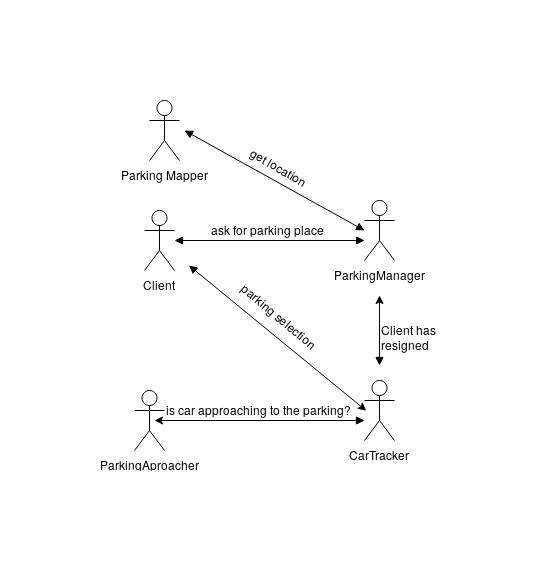
\includegraphics[width=1.0\linewidth]{interaction.png}
    \caption{Schemat interakcji.}
    \label{fig:interaction}
\end{figure}



%%%%%%%%%%%%%%%%%%%%%%%%%%%%%%%%%%%%%%%%%%%%%%%%%%%%%%%%%%%%%

\newpage
\subsection{Model agentów}

\begin{figure}[h!]
    \centering 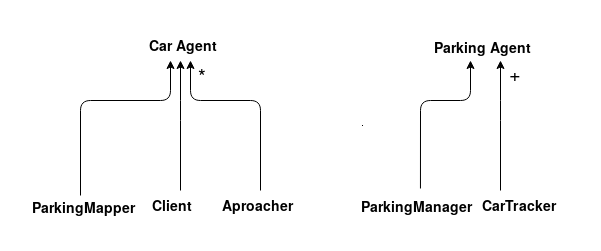
\includegraphics[width=1.0\linewidth]{agentmodel.png}
    \caption{Model agentów.}
    \label{fig:agentmodel}
\end{figure}

Na podstawie powyższych schematów (\ref{fig:agentmodel}) modeli agentów można stwierdzić, że oba rodzaje agentów  występujących w systemie są złożone w kontekście zaimplementowanych w nich ról. ParkingAgent posiada nieco większe skomplikowanie z uwagi na bardziej odpowiedzialną rolę jaką pełni w systemie, ponieważ to agenty-parkingi zarządzają agentami-pojazdami jednocześnie spełniając ich prośby. System nie może istnieć bez żadnej instancji ParkingAgent, ponieważ CarAgent w roli klienta nie mógłby wchodzić w interakcje i w rezultacie zaparkować. Natomiast można wyobrazić sobie istnienie systemu z instancjami ParkingAgent’a bez drugiego rodzaju agentów występujących w systemie.

\newpage
\subsubsection{Map Parkings}
\begin{table}[h]
    \centering
    \begin{tikzpicture}
    \node (a) at (0,0)
    {
        \begin{tabular}{|p{4cm}|p{4cm}|p{1cm}p{4cm}}
            \cline{1-2}
            \multicolumn{2}{|p{8cm}|}{UpdateParkingsCordinates (INFORM REF)} &  & \\ \cline{1-2}
            \textbf{ParkingMapper} & \textbf{ParkingManager} & \hspace{5mm}  & \\ \cline{1-3}
            \multicolumn{2}{|p{8cm}|}{Wysyła zapytania do wszystkich parkingów i uaktualnia ich położenie z prośbą o informacje o ich lokalizacji} & \hspace{5mm}  &  \\ \cline{1-3}
            \end{tabular}
    };
    \node[yshift=-2cm] (b) at (a.south) 
    {
        \begin{tabular}{|p{4cm}|p{4cm}|p{1cm}p{4cm}}
            \cline{1-2}
            \multicolumn{2}{|p{8cm}|}{SendCoordinates (INFORM)} &  & \\ \cline{1-2}
            \textbf{ParkingManager} & \textbf{ParkingMapper} & \hspace{5mm}  & \\ \cline{1-3}
            \multicolumn{2}{|p{8cm}|}{wysyła koordynaty parkingu} & \hspace{5mm}  &  parking\_location \\ \cline{1-3}
            \end{tabular}
    };
    \draw[->,ultra thick](a)--(b);
    \end{tikzpicture}
    \label{my-label}
    \end{table}

\subsubsection{PlaceReservation}
\begin{table}[h]
    \centering
    \begin{tikzpicture}
    \node (a) at (0,0)
    {
        \begin{tabular}{|p{4cm}|p{4cm}|p{1cm}p{4cm}}
            \cline{1-2}
            \multicolumn{2}{|p{8cm}|}{CallForParkingOffers (CallForProporsal)} &  & \\ \cline{1-2}
            \textbf{Client} & \textbf{Parking Manager} & \hspace{5mm}  & parking\_list \\ \cline{1-3}
            \multicolumn{2}{|p{8cm}|}{Wysyła prośbę o rezerwację miejsca postojowego do parkingów z wolnymi miejscami w określonej odległości} & \hspace{5mm}  &  \\ \cline{1-3}
            \end{tabular}
    };
    \node[yshift=-2cm] (b) at (a.south) 
    {
        \begin{tabular}{|p{4cm}|p{4cm}|p{1cm}p{4cm}}
            \cline{1-2}
            \multicolumn{2}{|p{8cm}|}{SendAvailablePlaceInfo (Propose)} &  & \\ \cline{1-2}
            \textbf{Parking Manager} & \textbf{Client} & \hspace{5mm}  &  \\ \cline{1-3}
            \multicolumn{2}{|p{8cm}|}{wysyła Clientowi informacje o dostępności miejsca, jeżeli takie posiada} & \hspace{5mm}  &  \\ \cline{1-3}
            \end{tabular}
    };
    \node[yshift=-2cm] (c) at (b.south) 
    {
        \begin{tabular}{|p{4cm}|p{4cm}|p{1cm}p{4cm}}
            \cline{1-2}
            \multicolumn{2}{|p{8cm}|}{AcceptParkingOffer (AcceptProposal)} &  & \\ \cline{1-2}
            \textbf{Client} & \textbf{Parking Manager} & \hspace{5mm}  &  \\ \cline{1-3}
            \multicolumn{2}{|p{8cm}|}{otrzymuje odpowiedź Clienta czy rezerwuje wskazane miejsce} & \hspace{5mm}  &  \\ \cline{1-3}
            \end{tabular}
    };
    \draw[->,ultra thick](a)--(b);
    \draw[->,ultra thick](b)--(c);
    \end{tikzpicture}
    \label{my-label}
    \end{table}


\newpage
\subsubsection{TrackCarWithReservation}
\begin{table}[h]
    \centering
    \begin{tikzpicture}
    \node (a) at (0,0)
    {
        \begin{tabular}{|p{4cm}|p{4cm}|p{1cm}p{4cm}}
            \cline{1-2}
            \multicolumn{2}{|p{8cm}|}{SendReservationInfo (INFORM)} &  & \\ \cline{1-2}
            \textbf{Approacher} & \textbf{CarTracker} & \hspace{5mm}  & parking\_list \\ \cline{1-3}
            \multicolumn{2}{|p{8cm}|}{przekazuje dane rezerwacji do Car Trackera po akceptowaniu wskazanego miejsce} & \hspace{5mm}  &  \\ \cline{1-3}
            \end{tabular}
    };
    \node[yshift=-2cm] (b) at (a.south) 
    {
        \begin{tabular}{|p{4cm}|p{4cm}|p{1cm}p{4cm}}
            \cline{1-2}
            \multicolumn{2}{|p{8cm}|}{SubscribeForClientLocation (Subscribe)} &  & \\ \cline{1-2}
            \textbf{CarTracker} & \textbf{Approacher} & \hspace{5mm}  &  \\ \cline{1-3}
            \multicolumn{2}{|p{8cm}|}{prosi Approachera o cykliczne wysyłanie swojej lokalizacji} & \hspace{5mm}  &  \\ \cline{1-3}
            \end{tabular}
    };
    \node[yshift=-2cm] (c) at (b.south) 
    {
        \begin{tabular}{|p{4cm}|p{4cm}|p{1cm}p{4cm}}
            \cline{1-2}
            \multicolumn{2}{|p{8cm}|}{SendApproacherLocation (inform)} &  & \\ \cline{1-2}
            \textbf{Approacher} & \textbf{CarTracker} & \hspace{5mm}  &  \\ \cline{1-3}
            \multicolumn{2}{|p{8cm}|}{wysyła cyklicznie dane o swojej lokalizacji do Car Trackera} & \hspace{5mm}  & ApproacherIsNotComing \\ \cline{1-3}
            \end{tabular}
    };
    \draw[->,ultra thick](a)--(b);
    \draw[->,ultra thick](b)--(c);
    \end{tikzpicture}
    \label{my-label}
    \end{table}

\subsubsection{ReservationCancellation}
\begin{table}[h]
    \centering
    \begin{tikzpicture}
    \node (a) at (0,0)
    {
        \begin{tabular}{|p{4cm}|p{4cm}|p{1cm}p{4cm}}
            \cline{1-2}
            \multicolumn{2}{|p{8cm}|}{CancelClientReservation (CANCEL)} &  & \\ \cline{1-2}
            \textbf{Approacher} & \textbf{CarTracker} & \hspace{5mm}  & parking\_list \\ \cline{1-3}
            \multicolumn{2}{|p{8cm}|}{wysyła informacje o rezygnacji z miejsca parkingowego } & \hspace{5mm}  & AproacherCancelledReservation \\ \cline{1-3}
            \end{tabular}
    };
    \node[yshift=-2cm] (b) at (a.south) 
    {
        \begin{tabular}{|p{4cm}|p{4cm}|p{1cm}p{4cm}}
            \cline{1-2}
            \multicolumn{2}{|p{8cm}|}{ConfirmCancellation (Confirm)} &  & \\ \cline{1-2}
            \textbf{CarTracker} & \textbf{Approacher} & \hspace{5mm}  &  \\ \cline{1-3}
            \multicolumn{2}{|p{8cm}|}{potwierdza otrzymanie informacji o rezygnacji} & \hspace{5mm}  & AproacherCancelledReservation \\ \cline{1-3}
            \end{tabular}
    };
    \draw[->,ultra thick](a)--(b);
    \end{tikzpicture}
    \label{my-label}
    \end{table}


\newpage
\subsubsection{FreePlace}
\begin{table}[h]
    \centering
    \begin{tikzpicture}
    \node (a) at (0,0)
    {
        \begin{tabular}{|p{4cm}|p{4cm}|p{1cm}p{4cm}}
            \cline{1-2}
            \multicolumn{2}{|p{8cm}|}{RequestSetPlaceFree (Request)} &  & \\ \cline{1-2}
            \textbf{CarTracker} & \textbf{Parking Controller} & \hspace{5mm}  & parking\_list \\ \cline{1-3}
            \multicolumn{2}{|p{8cm}|}{wysyła żądanie usunięcia rezerwacji miejsca do Parking Controllera} & \hspace{5mm}  & \\ \cline{1-3}
            \end{tabular}
    };
    \node[yshift=-2cm] (b) at (a.south) 
    {
        \begin{tabular}{|p{4cm}|p{4cm}|p{1cm}p{4cm}}
            \cline{1-2}
            \multicolumn{2}{|p{8cm}|}{ConfirmFreedPlace (Confirm)} &  & \\ \cline{1-2}
            \textbf{Parking Controller} & \textbf{CarTracker} & \hspace{5mm}  &  \\ \cline{1-3}
            \multicolumn{2}{|p{8cm}|}{potwierdza otrzymanie informacji o rezygnacji} & \hspace{5mm}  & AproacherCancelledReservation \\ \cline{1-3}
            \end{tabular}
    };
    \draw[->,ultra thick](a)--(b);
    \end{tikzpicture}
    \label{my-label}
    \end{table}

%%%%%%%%%%%%%%%%%%%%%%%%%%%%%%%%%%%%%%%%%%%%%%%%%%%%%%%%%%%%%

\newpage
\subsection{Model usług}

\hyphenation{Approacher-Is-Not-Coming}

\begin{table}[!h] \label{tab:modeluslug} \centering
    \caption{Model usług.}
    \begin{tabular} {| m{2cm} | m{2cm} | m{3cm} | m{3cm} | m{4cm} |} \hline
        Usługa   & Wejścia & Wyjścia & Warunki wstępne & Warunki końcowe \\ \hline
        Tworzenie listy parkingów & - & parking\_list & true & parking\_list =/= NULL \\ \hline
        Znalezienie wolnego miejsca & car\_location & reservation\_info & parking\_list =/= NULL & reservation\_info =/= NULL \\ \hline
        Śledzenie położenia samochodu & car\_location reservation\_info & ApproacherIsNot\-Coming & reservation\_info =/= NULL & ApproacherIsNot\-Coming = True OR IsApproacher = False \\ \hline
        Odwoływanie zarezerwowanego miejsca & reserva\-tion\_info & Approacher\-Cancelled\-Reservation & reservation\_info =/= NULL & ApproacherCancelled\-Reservetation = True \\ \hline
    \end{tabular}
\end{table}

%%%%%%%%%%%%%%%%%%%%%%%%%%%%%%%%%%%%%%%%%%%%%%%%%%%%%%%%%%%%%


\newpage
\subsection{Model znajomości}

\begin{figure}[h!]
    \centering 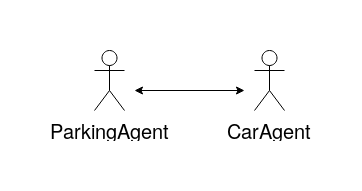
\includegraphics[width=1.0\linewidth]{friends.png}
    \caption{Model znajomości.}
    \label{fig:friends}
\end{figure}

Model znajomości agentów w systemie (Rys. \ref{fig:friends}) jest nieskomplikowany z uwagi na małą liczbę agentów w nim występujących. Wszystkie rodzaje agentów komunikują się między sobą. Nadmienić należy że architektura systemu została zaprojektowana w ten sposób, że nie wymaga komunikacji pomiędzy różnymi instancjami tego samego rodzaju agenta. W ParkingAgent następuje komunikacja pomiędzy rolami, w które wciela się ta sama instancja tego rodzaju genta.
\newpage
\section{Opis implementacji systemu}

\subsection{Framework}
Framework
Narzędziem użytym w realizacji projektu jest JADE 4.5.0 (Java Agent Development Framework). Jest to popularny framework przeznaczony do implementowania systemów wieloagentowych w pełni zaimplementowany w języku Java. Wybraliśmy JADE, ponieważ jak można przeczytać w dokumentacji:

\begin{itemize}
\item w JADE wdrożony został pełny model komunikacji FIPA, a jego komponenty zostały wyraźnie wyróżnione i w pełni zintegrowane: protokoły interakcji, koperta, ACL, języki treści, schematy kodowania, ontologie i protokoły transportowe. 

\item architektura komunikacji oferuje elastyczne i wydajne przesyłanie wiadomości, gdzie JADE tworzy i zarządza kolejką przychodzących wiadomości ACL. Agenci mogą uzyskać dostęp do swojej kolejki za pomocą kombinacji kilku trybów: blokowania, odpytywania, limitu czasu i dopasowywania wzorców. 

\item Dodatkowo przydatną funkcjonalnością jest możliwość sterowania konfiguracją za pomocą interfejsu GUI. 
\end{itemize}

\subsection{Sposób implementacji agentów}
Utworzyliśmy dwie klasy agentów CarAgent oraz ParkingAgent. Każdy agent dziedziczy funkcjonalność po klasie jade.core.Agent. Agenty wykorzystują klasę jade.core.behaviours.
Behaviour do implementacji aktywności oraz protokołów zdefiniowanych dla ról. 

\textbf{CarAgent} - Agent samochód, który może się przemieszczać. Dla celów testowych przyjęliśmy, iż na początku swojego istnienia agent ten losuje swoją pozycję początkową na mapie i dodaje zachowania UpdateListOfParkings, CallForParkingOffers, SendReservationInfo oraz ReservationCancellation, ListenForLocationCancelSubscriptionFromCarTracker.

\textit{UpdateListOfParkings} - służy do  wysyłania zapytania do wszystkich parkingów z prośbą o informacje o ich lokalizacji i uaktualnienia ich położenia. Protokół ten jest aktywowany na początku istnienia agenta samochodu. Agent zapisuje położenia wszystkich parkingów w HashMapie, gdzie kluczem jest AID parkingu, a wartością jest lokalizacja parkingu. Lokalizacje wszystkich parkingów są niezbędne dla CarAgent, ponieważ chce on wiedzieć, który parking dysponujący wolnym miejscem znajduje się najbliżej. 

\textit{CallForParkingOffers} - służy do zapoczątkowania konwersacji z najbliższymi parkingami w celu zarezerwowania miejsca. Agent samochód wysyła wiadomość typu CFP i otrzymuje od parkingów posiadających wolne miejsce odpowiedź typu PROPOSE lub REFUSE. Następnie typowany jest najbliższy parking z wolnym miejscem i podejmowana jest próba dokonania rezerwacji miejsca (ACCEPT PROPOSAL). Jeżeli CarAgent otrzyma odpowiedź pozytywną (INFORM) od ParkingAgent, to dany parking jest zapisany w pamięci jako cel podróży, jeżeli jednak otrzymamy odpowiedź negatywną (FAILURE) to ponownie rozpoczynamy protokół CallForParkingOffers.

\textit{SendReservationInfo} - służy do wysłania wiadomości od CarAgent (INFORM) do ParkingAgent o rezerwacji zrobionej dla konkretnego agenta. Po otrzymaniu informacji ParkingAgent wysyła potwierdzenie CONFIRM.

\textit{CancelClientReservation} - służy do wysłania wiadomości o rezygnacji z zarezerwowanego miejsca (CANCEL) do ParkingAgent, będącego do tej pory celem podróży agenta-samochodu (CarAgent). Po otrzymaniu takiego żądania ParkingAgent zwalnia miejsce postojowe, a następnie wysyła potwierdzenie wykonania akcji (CONFIRM).

\textit{ListenForLocationCancelSubscriptionFromCarTracker} - służy do nasłuchiwania czy CarTracker chce przestać subskrybować wiadomości, które są wysyłane w protokole SendReservationInfo.


\textbf{ParkingAgent} - agent parking posiadający miejsca parkingowe udostępniane pojazdom. Głównym zadaniem agenta jest oferowanie wolnych miejsc parkingowych oraz śledzenie aktualnej pozycji samochodów posiadających rezerwację. Agent ten wykorzystuje zachowania:

\textit{SendCoordinates} - służy do wysłania informacji o swojej pozycji. Zachowanie to jest cykliczne i wykonywane po otrzymaniu wiadomości od agenta samochodu typu INFORM\_REF.

\textit{SendAvailablePlaceInfo} - zachowanie to jest cykliczne, wykonywane po przyjściu wiadomości zawierającej performatywę CFP od CarAgent. Jeżeli agent posiada wolne miejsce parkingowe to wysyła wiadomość typu PROPOSE w odpowiedzi. W przypadku kiedy agent nie posiada wolnego miejsca następuje wysłanie odpowiedzi zawierającej performatywę REFUSE.

\textit{ConfirmReservation} - zachowanie cykliczne; po otrzymaniu od CarAgent wiadomości zawierającej performatywę ACCEPT\_PROPOSAL, wyrażającej chęć zarezerwowania miejsca na danym parkingu, ParkingAgent zmienia stan miejsca z “wolny” na “zajęty” i odsyła wiadomość o pozytywnym przebiegu procesu (INFORM). Jeśli dane miejsce zostanie przed otrzymaniem wiadomości zawierającej ACCEPT\_PROPOSAL zajęte przez innego CarAgent, zostaje wysłana wiadomość informująca o niepowodzeniu rezerwacji (FAILURE).

\textit{ConfirmCancellation} - zachowanie cykliczne, po otrzymaniu wiadomości od CarAgent wyrażającej żądanie usunięcia rezerwacji miejsca parkingowego (CANCEL) zmienia stan miejsca z “zajęty” na “wolny”, a następnie wysyła odpowiedź o powodzeniu akcji (CONFIRM).

\textit{getReservationInfo} - zachowanie cykliczne; służy do odbierania wiadomości od CarAgent o dokonaniu rezerwacji dla tego CarAgenta na parkingu, którym jest adresat wiadomości - ParkingAgent. Po otrzymaniu informacji ParkingAgent przesyła potwierdzenie CONFIRM.


\subsection{Sposób implementacji komunikatów}

\subsubsection{Zastosowane performatywy}
\begin{enumerate}
    \item INFORM\_REF
    \item INFORM
    \item FAILURE
    \item CFP
    \item PROPOSE
    \item ACCEPT\_PROPOSAL
    \item CANCEL
    \item CONFIRM
    \item REFUSE
\end{enumerate}

\subsubsection{Protokoły komunikacyjne}

W trakcie dotychczasowej implementacji został użyty tylko jeden typowy protokół komunikacyjny zdefiniowany przez FIPA i jest nim Subscribe Interaction Protocol, który został zastosowany do śledzenia Car Agents przez rolę CarTracker realizowaną przez Parking Agent. Pozostała wymiana komunikatów pomiędzy agentami została zebrana w indywidualnie zdefiniowanych dla naszego systemu protokołach stworzonych poprzez rozszerzenie klasy Behaviours, CyclicBehaviours oraz TickerBehaviours.

\subsubsection{Zastosowane języki treści}
Zastosowanym językiem treści jest FIPA Semantic Language (SL), który jest standardowo zaimplementowany we frameworku JADE.

\subsection{Wykorzystane standardy}

Implementowany system jest zgodny ze standardami FIPA, ze względu na wykorzystanie frameworka JADE.

\begin{itemize}
\item FIPA ACL (Agent Communication Language)
\item FIPA SL (Semantic Language) - język semantyczny dla komunikacji ACL

\end{itemize}


\subsection{Algorytmy}

Algorytmy wykorzystane w systemie zostały pokrótce opisane w sposobie implementacji agentów. Na uwagę zasługuje sposób implementacji środowiska oraz sposób poruszania się po nim agentów. Stan naszego systemu jest zdefiniowany w postaci mapy 2D, gdzie każda z kratek odpowiada współrzędnej w środowisku agentów. Do każdej współrzędnej mogą być przypisane trzy wartości: czy współrzędna jest ulicą czy parkingiem. Samochody są losowo inicjalizowane na współrzędnych odpowiadających ulicom. Parking docelowy jest znajdowany poprzez obliczanie ścieżek do wszystkich parkingów, a następnie wybranie najkrótszej trasy. Samochód porusza się w jego kierunku po drodze obliczonej w algorytmie wybierania ścieżki (opisanym poniżej). Końcowo samochód wjeżdża na współrzędną z parkingiem. Dopuszcza się możliwość, że dwa samochody znajdują się na tej samej współrzędnej. W aktualnej wersji systemu wszystkie pola mapy są ulicami.

\textbf{Algorytm wyznaczania ścieżki} został zaimplementowany przy pomocy algorytmu przeszukiwania wszerz (BFS). Algorytm ten w formie iteracyjnej wykorzystuje kolejkę do określenia, które kolejne punkty powinniśmy przebadać. Rozpoczynając od punktu startowego dodajemy wszystkie sąsiednie, nieodwiedzone wcześniej, punkty do kolejki i powtarzamy ten proces dla wszystkich punktów w kolejce. Jeżeli dotrzemy do punktu docelowego to zwracamy listę, która jest ścieżką od miejsca początkowego do docelowego. Nie jest to najoptymalniejszy algorytm (u nas, O($ i \cdot j $) time | O($ i \cdot j $) space, gdzie i - szerokość mapy, j - wysokość mapy), jednak został wybrany ze względu na łatwość implementacji w realizowanym systemie.

\newpage
\subsection{Wizualizacja}

Postanowiliśmy zwizualizować działanie naszego projektu poprzez wyświetlanie informacji o aktualnym stanie systemu w konsoli oraz pokazywaniu położenia agentów na mapie 2D. Agent aktualizując swoje położenie wysyła informację do serwera, który przechowuje dane o bieżącym położeniu każdego agenta. Następnie serwer przekazuje uaktualnione informacje do aplikacji React, gdzie wyświetlana jest mapa. Backend i Frontend połączone są ze sobą poprzez websocket, więc wszystkie aktualizacje są wykonywane w czasie rzeczywistym. Ze względu na taki stos technologiczny możliwe są opóźnienia pomiędzy prezentowanym stanem systemu na mapie, a w konsoli. Przykładowa mapa jest widoczna na rysunku \ref{fig:przyklad_mapy}, gdzie kratka: biała oznacza drogę, czerwona parking, a niebieska samochód. Przykładowe wizualizacje naszego systemu są dostępne w postaci gifów na repozytorium naszego projektu w README.

\begin{figure}[H]
    \centering 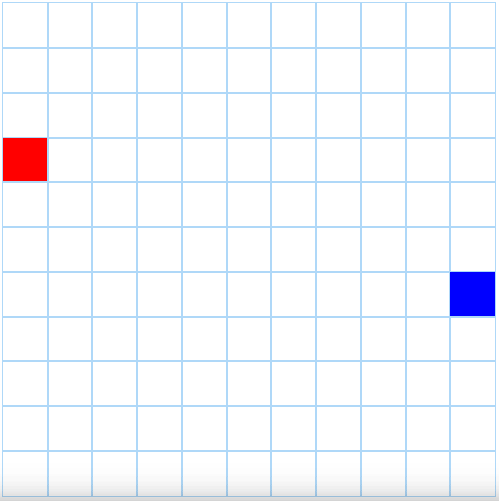
\includegraphics[width=0.7\linewidth]{przyklad_mapy.png}
    \caption{Przykład mapy.}
    \label{fig:przyklad_mapy}
\end{figure}

\newpage
\subsection{Napotkane problemy i zmiany w kolejnej iteracji}
\begin{itemize}
\item Żaden członek zespołu nie jest biegły w Javie, więc dodatkową trudnością  było szybkie zapoznanie się z samym językiem, a nie tylko nowym frameworkiem. Z tego powodu, nie mogliśmy się wyłącznie skupić na najlepszym rozwiązaniu i implementacji problemu.

\item Podczas implementacji równoległego oczekiwania na wiadomości mieliśmy problem z przechwytywaniem wiadomości przez niepowołane do tego zachowania. Problem ten rozwiązaliśmy wykorzystując zaimplementowane w JADE szablony wiadomości (jade.lang.acl.MessageTemplate). Za pomocą metod MatchPerformative, MatchConversationID i wyfiltrowaliśmy przychodzące wiadomości skierowane do poszczególnych zachowań.
\end{itemize}
\clearpage
\newpage
%--------------------------------------------
% Literatura
%--------------------------------------------


\printbibliography

%--------------------------------------------
% Spisy (opcjonalne)
%--------------------------------------------
\newpage

% Wykaz symboli i skrótów.
% Pamiętaj, żeby posortować symbole alfabetycznie
% we własnym zakresie. Ponieważ mało kto używa takiego wykazu, 
% uznałem, że robienie automatycznie sortowanej listy
% na poziomie LaTeXa to za duży overkill. 
% Jest tylko proste i oczywiste makro \acronym, 
% które dodaje postawowe formatowanie. 
% //AB
% \vspace{0.8cm}
% \section*{Wykaz symboli i skrótów}
% \acronym{EiTI}{Wydział Elektroniki i Technik Informacyjnych}
% \acronym{PW}{Politechnika Warszawska}

\listoffigures              % Spis obrazków. 
\vspace{1cm}                % vertical space
\listoftables               % Spis tabel. 
\vspace{1cm}                % vertical space


% \listofappendices           % Spis załączników
% Załączniki
% \appendix

% \newpage
% \newappendix{Nazwa załącznika 1}
% \lipsum[1]

% \newpage
% \newappendix{Nazwa załącznika 2}
% \lipsum[1]

% Używając powyższych spisów jako szablonu,
% możesz tu dodać swój własny wykaz bądź listę, 
% np. spis algorytmów. 

\end{document} % Dobranoc. 

